%\documentclass{article}
\documentclass[oneside]{report} 

\usepackage[UTF8, fntef]{ctex}
\usepackage{graphicx}
\usepackage{epstopdf}

%\usepackage[a4paper, total={6in, 10in}]{geometry}
\usepackage[left=2cm,right=4.cm,top=2cm,bottom=2cm]{geometry} 
%\usepackage{setspace}
%\singlespacing
%\onehalfspacing
%\doublespacing

\usepackage[backref]{hyperref} 
\usepackage{amsmath}
\usepackage{booktabs} % 导入三线表需要的宏包
\usepackage{caption}
\usepackage{float} 
%
\usepackage{subfigure}
%\usepackage{subcaption}
\usepackage[numbers,sort&compress]{natbib}%参考文献顺序
\usepackage{siunitx}%\SI{}{\degreeCelsius}
\hypersetup{hidelinks}



%----------------------------------------------
%----------------------------------------------
%
\usepackage{amssymb}
\usepackage{amsfonts}


\usepackage{color, xcolor}
\usepackage{soul}


\usepackage{hyperref}
%
\hypersetup{
    colorlinks=true,
    linkcolor=magenta, %blue,
    filecolor=black, %magenta,      
    urlcolor=blue, %blue, %cyan,
    pdftitle={Sharelatex Example},
    bookmarks=true,
    %pdfpagemode=FullScreen,
    linktoc=all  %set to all if you want both sections and subsections linked
}


% todonotes
\usepackage[colorinlistoftodos,
%textsize=scriptsize,
bordercolor=white
%, textcolor=orange!80!black!100
, color=lime!33
]{todonotes}
\setlength{\marginparwidth}{3.4cm}
\newcommand{\donein}{\todo[color=blue!11,inline]}
\newcommand{\done}{\todo[color=blue!11]}

%----------------------------------------------
%----------------------------------------------



\begin{document}


\chapter*{学习报告20231025}

本月阅读文献的主要目标,是寻找适合写综述的主题和方向。上月阅读的七篇综述中,1篇概述了储热技术的各个方面,1篇重点总结化学储热的研究,其余文章都专注一个小类别:3篇关于化学蓄热材料,1篇关于化学储热系统,1篇关于化学热泵技术。为了写出较为新颖的综述,可以关注化学储热技术中更小的分支。

在关于化学蓄热的材料的研究中,最多被提到的一类是金属盐或氢氧化物的水合物,及其用掺杂等方式制成的新型复合材料。研究这种复合材料的过程通常作为综述中大篇幅的一章,可以在进一步调查整理后形成一篇新的综述。而这些水合物中,出现频次最多的是$\mathrm{LiOH, CaCl_2}$和$\mathrm{Mg(OH)_2} $,于是我检索了每一种新型水合物(复合)材料发表的论文,以及针对这种材料作的综述文章,以对比研究性论文与综述论文的数量,结果见图\ref{tab:论文统计}。可以看出,$\mathrm{CaCl_2}$、$\mathrm{LiCl}$、$\mathrm{Mg(OH)_2}$和$\mathrm{MgCl_2}$相关的研究性论文数量远大于综述论文。

\begin{figure}[H]
    \centering
    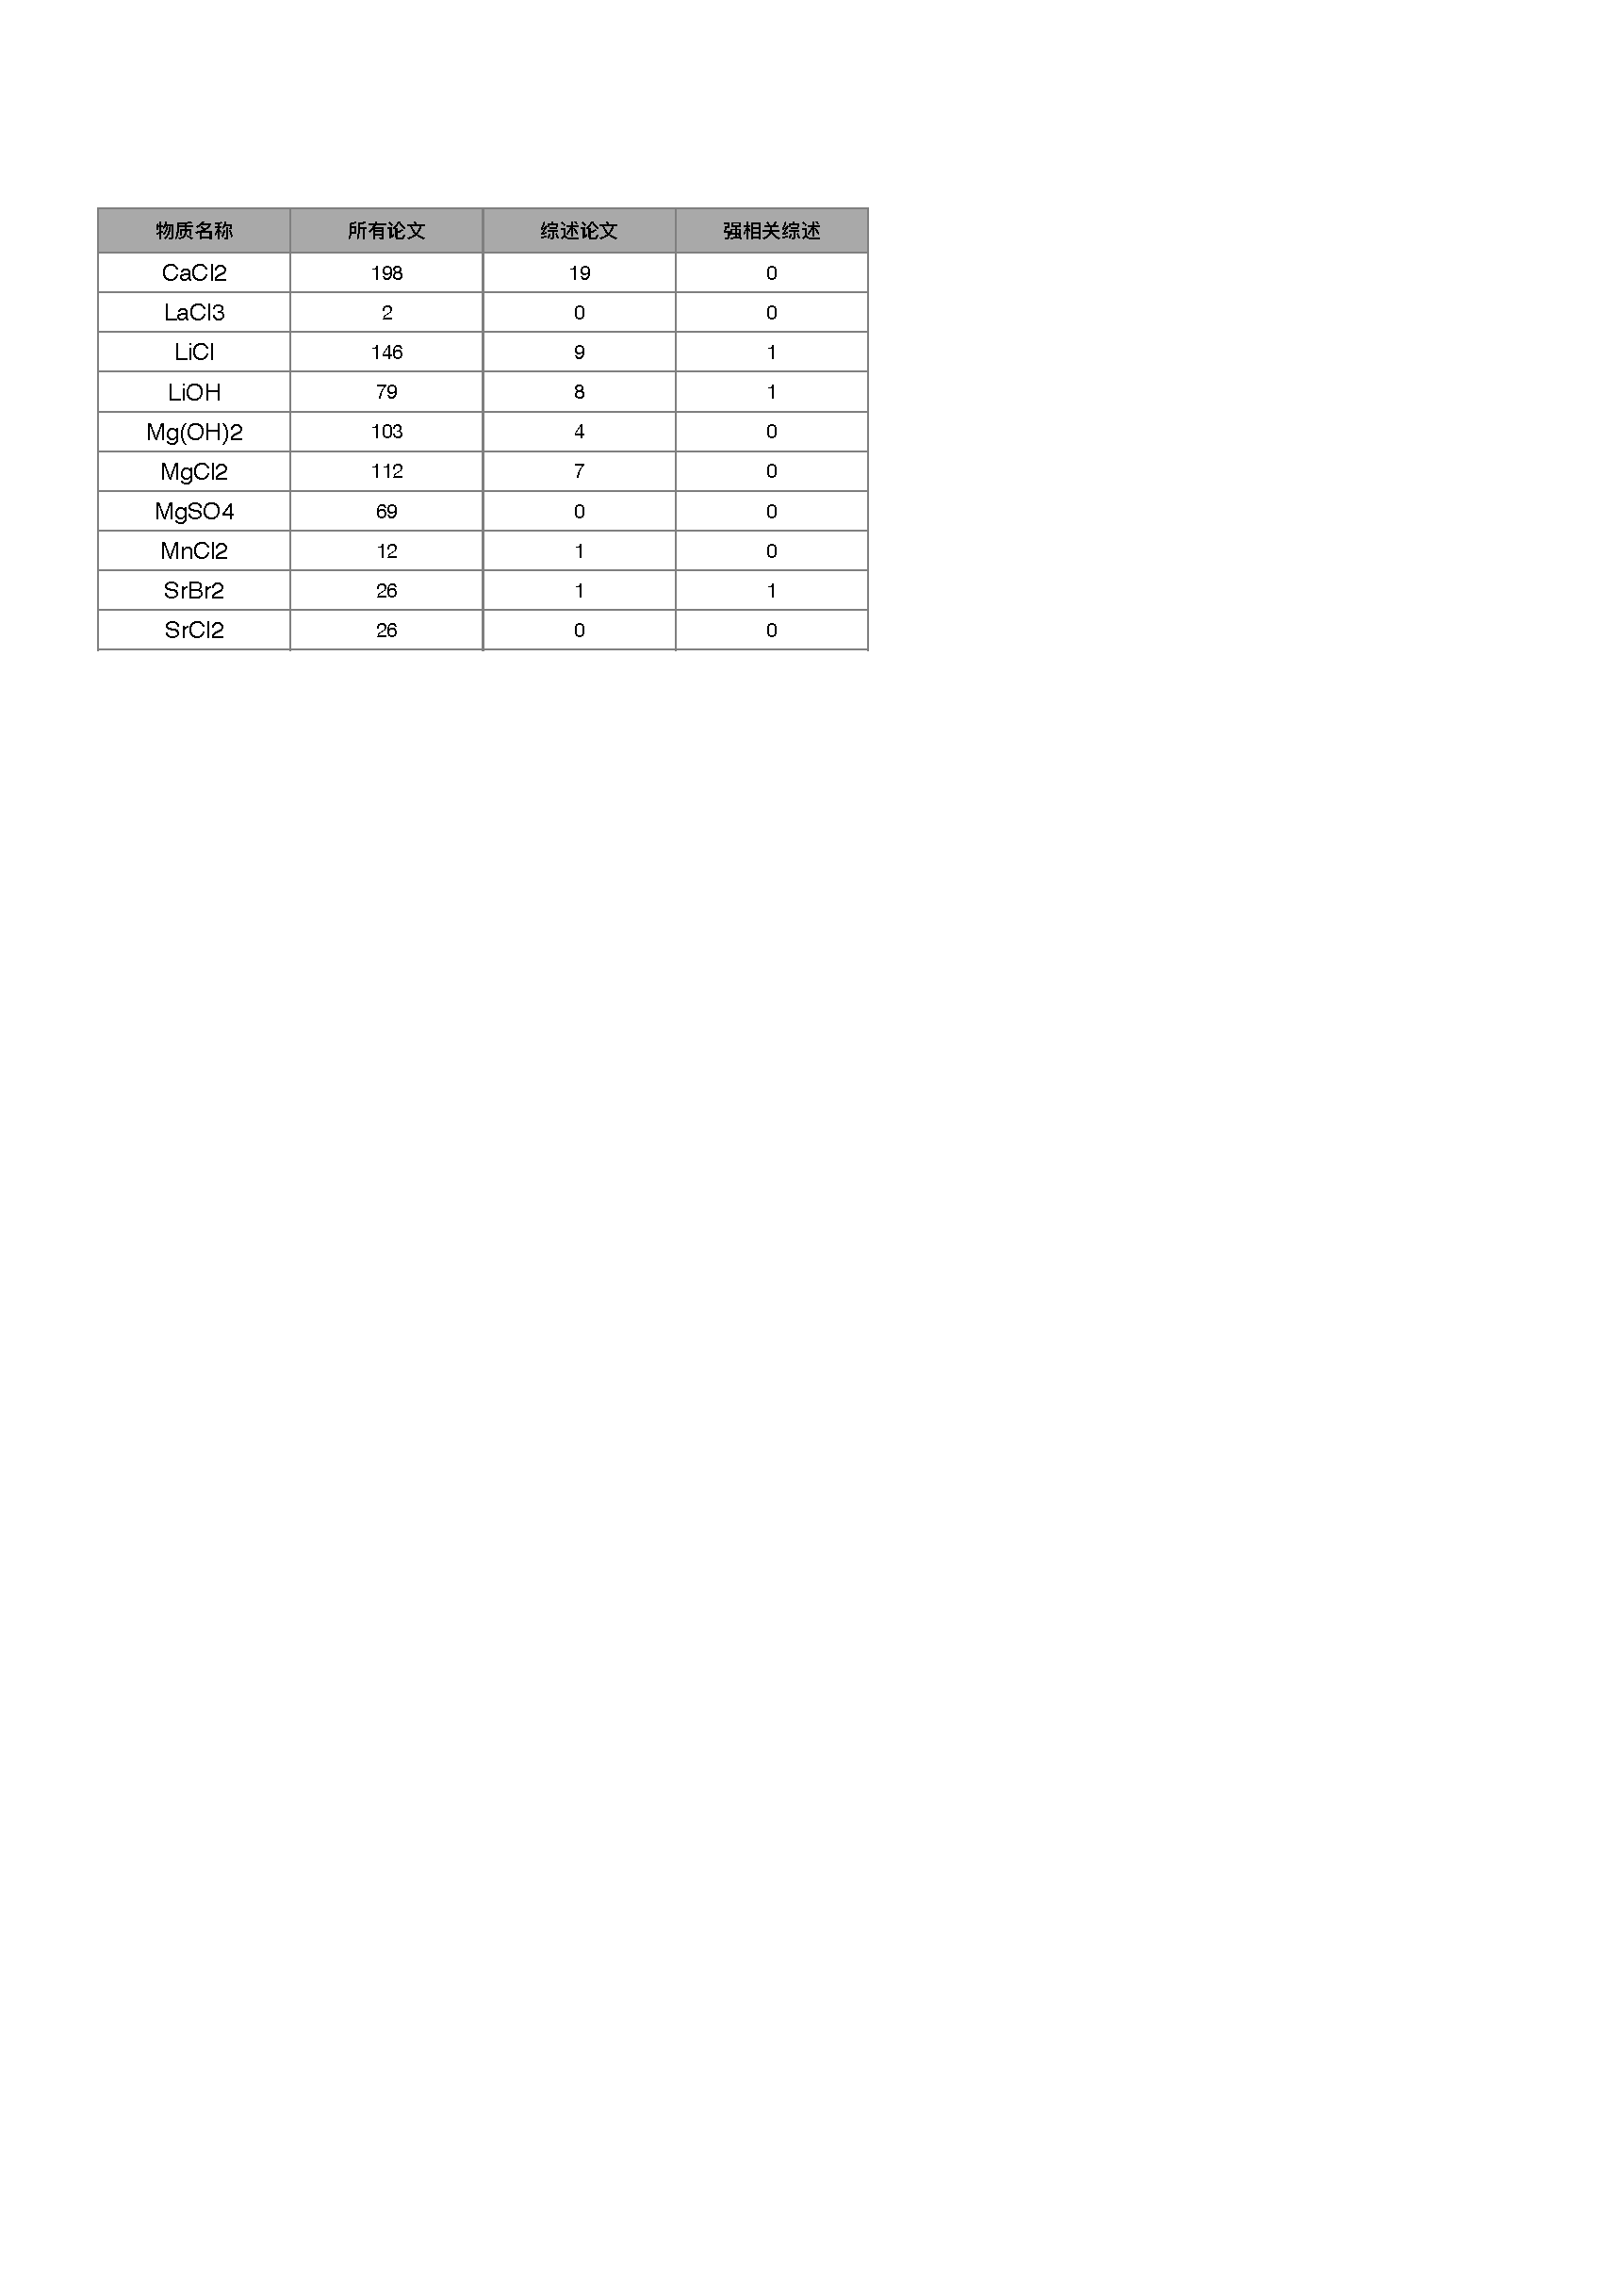
\includegraphics[width=0.9\textwidth]{image/论文统计.pdf}
    \caption{对于特定物质的研究性论文和综述论文数量比较}
    \label{tab:论文统计}
\end{figure}

在所有的综述论文中,最具有参考价值的是\href{https://doi.org/10.1016/j.rser.2021.111381}{\color{blue}《Lithium compounds for thermochemical energy storage: A state-of-the-art review and future trends》}\textsuperscript{\cite{RN126}}。这篇文章对锂化合物用于化学储热的各项研究进行了梳理,其主要内容见图\ref{fig:锂化合物}。除了该文章提到的各种技术外,近年来还有更多类似研究,例如利用高孔隙生物炭固定LiOH纳米颗粒\textsuperscript{\cite{RN48}},LiOH-金属有机框架衍生多孔碳复合材料用于储热\textsuperscript{\cite{RN49}}等,可以进行更新和扩充,形成一篇新的综述。同时,关于Ca或者Mg化合物的研究也可以形成一篇较新颖的综述。

\begin{figure}[H]
    \centering
    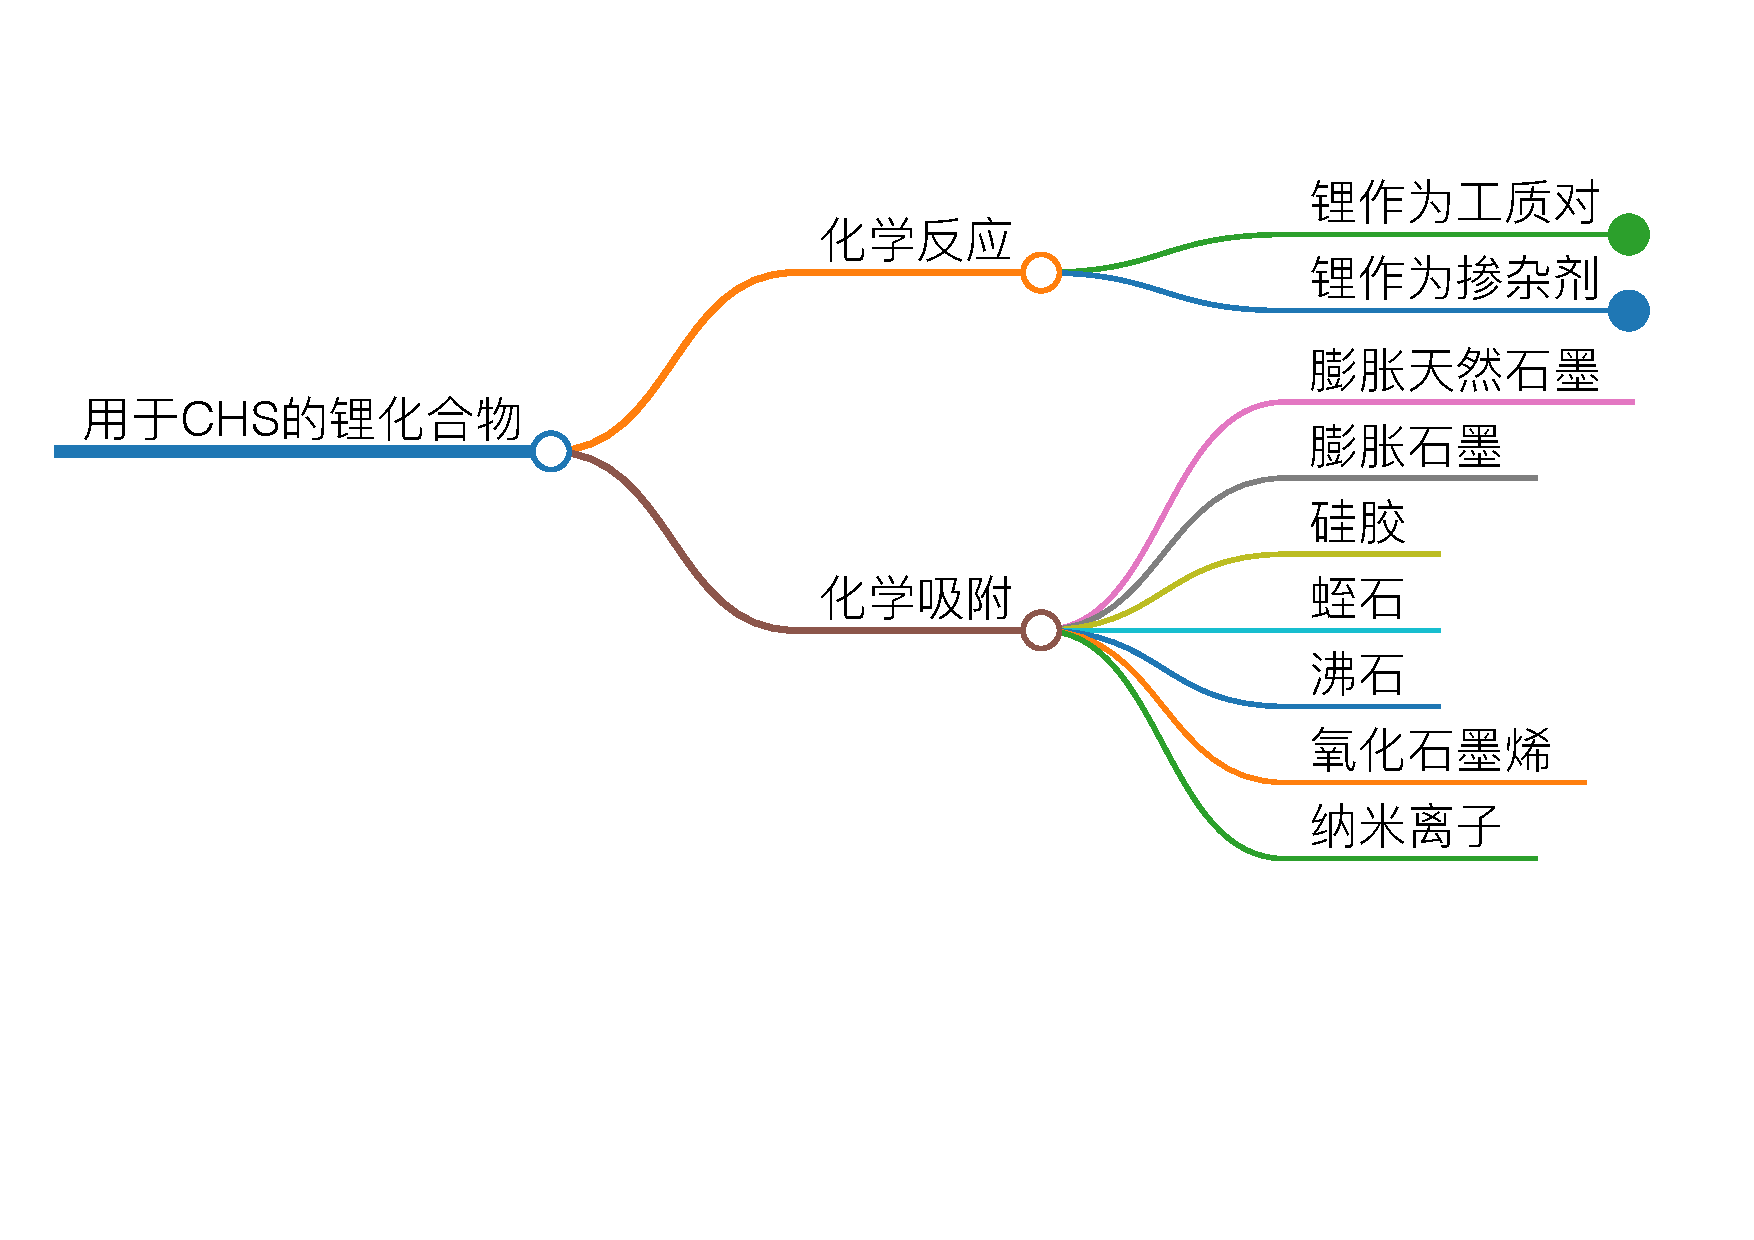
\includegraphics[width=0.7\textwidth]{image/锂化合物.pdf}
    \caption{锂化合物用于热化学储热的各方面研究}
    \label{fig:锂化合物}
\end{figure}




\bibliographystyle{IEEEtran}
\bibliography{cite.bib}

\end{document}
